%%%%%%%%%%%%%%%%%%
% 			 
%			Master Thesis - UWB
%				State of the art code
%
%			Author : Wilson Daubry
%
%%%%%%%%%%%%%%%%%%

\chapter{State of the art}
\label{stateoftheart}

This sections has the purpose to explain the state of the art.

\section{Ultra-Wideband Technology}

\gls{uwb} is a communication technology using, as the name states, a large bandwidth. This is not a new technology as it is the one used by  Guglielmo Marconi for the first transatlantic communication using radio waves \cite{nekoogar2005uwb}. As define by the \gls{itu-r} to be considered as \gls{uwb}, the bandwidth of communication must be at least 20 \% of the arithmetic center frequency \cite{itur2006characteristics}.

One interesting feature of \gls{uwb} is the possible coexistence with other radio waves already present in the environment such as \gls{wifi}. As it can be seen on Fig. \ref{fig:UWB_Techonology}, the extension of the \gls{uwb} in the spectral domain is quite huge. 

\begin{figure}[H]
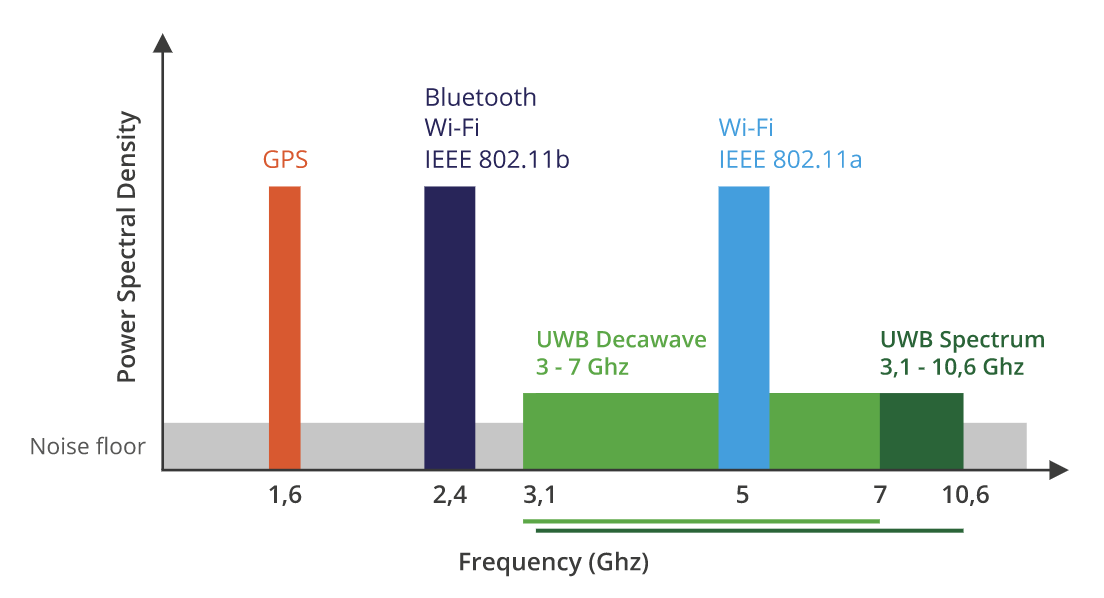
\includegraphics[width=.6\linewidth]{Images/uwb_bandwidth.png}
\centering
\caption{UWB spectrum compared to Wi-Fi and other wireless technology. Taken from \cite{itur2006characteristics}}
\label{fig:UWB_Techonology}
\end{figure} 

Knowing this and based on the time-frequency duality reminded in eq. \ref{fig:eq}, one can see that the extension in the time domain will be quite small.

\begin{equation}
	x(at) \longleftrightarrow \frac{1}{|a|}*X(\frac{f}{a})
\label{fig:eq}
\end{equation}

HERE - ADD THE IMAGE FOR TIME EXTENSION OF UWB

The Fig. \ref{fig:UWB_time} shows the theoretical duration of an impulse of the \gls{uwb}. An advantage of the \gls{uwb} is its robustness in regard of the \gls{mpc}. This can be understood by looking at Fig. \ref{fig:UWB_MPC_Theo}, where peaks several peaks can be distinguished, each corresponding either to a different path travelled by the wave. Indeed, the probability to have a collision depends on the size of the pulse sent. 

\section{Real Time Locating Systems}

\gls{rtls} are systems used to track and identify the location of objects in real time. This is a rather vague definition since nothing is specified concerning the means employed to achieve the localization. The \gls{rtls} that will be presented in this section will all have in common the use of wireless communications, between devices being called in this paper "anchor" and "tag". The tag being associated with the object to locate while the anchor is at a fixed and known location.

Those \gls{rtls} can be separated in two categories : "Relative localization" and "Absolute localization". The only relative localization algorithm presented in \ref{sds2wr} is the \gls{tof} method that is used in this project to compute the distance between an anchor and a tag. This choice has been made and explained in \cite{fesler2018high}, \cite{hannotier2019indoor} along a presentation all several approach to determine the relative position of a tag relatively to an anchor.

% Faire un lien vers la Thèse de Quentin F entre autre où tout est déjà expliqué et résumé brièvement l'idée.

\subsection{Symmetric double sided two-way ranging}
\label{sds2wr}

\gls{sdstwr} consists in an exchange of three messages between two devices, respectively $RDEV_1$ initiating the communication and `$RDEV_2$. Each device need to save the \gls{toe} or \gls{toa} of every message. Those time being respectively $t_0$, $t_1$ for the first message, $t_2$, $t_3$ for the second message and $t_4$, $t_5$ for the last message.

Each message contains the different timestamps previously computed, meaning that at the end of this exchange $RDEV_2$ possess all the informations about the timestamps, while $RDEV_1$ misses the last one. If one wants $RDEV_1$ to be able to compute the \gls{tof} then a last message with that $t_5$ in it should be exchanged.

A scheme of \gls{sdstwr} is shown on Fig. \ref{sdstwr}. 

\begin{figure}[H]
\centering
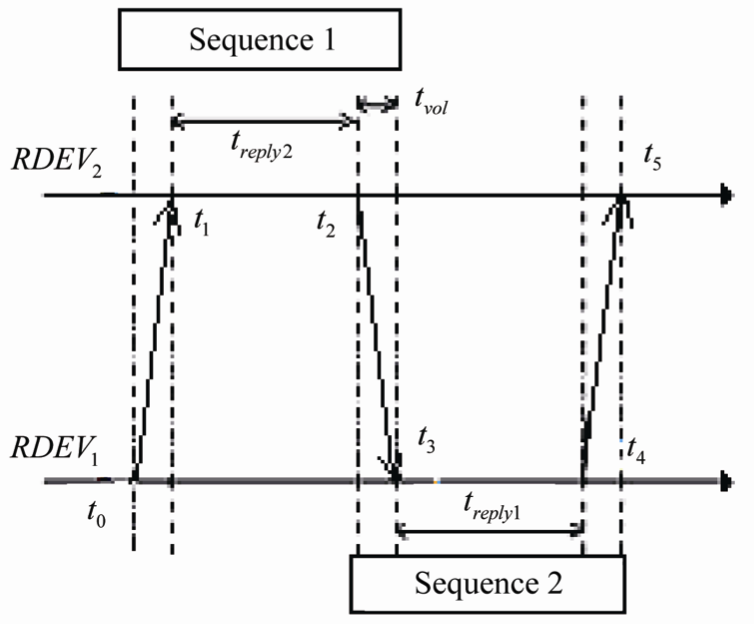
\includegraphics[width=.6\linewidth]{Images/sds-twr.png}
\caption{Symmetric double-sided two-way ranging. Taken from \cite{dalce2011comparison}}
\label{sdstwr}
\end{figure}

Based on those timestamps, the computation of the \gls{tof} can be observed in eq. \ref{fig:tof}.

\begin{equation}
	t_{est} = \frac{((t_3 - t_0) - (t_2 - t_1)) + ((t_5 - t_2) - (t_4 - t_3))}{4}
\label{fig:tof}
\end{equation}

Since that \gls{tof} computed remains an estimation, it is important to know the magnitude of the error as well as its evolution in parallel of the true value of the \gls{tof}.

\begin{equation}
	t_{true} - t_{est} = \frac{1}{4}*(t_{reply2} - t_{reply_1})*(e_1 - e_2)
\end{equation}

\subsection{Trilateration}

% Rappeler le concept avec un schéma concis. 

\section{Project advancement}

% L'objectif de cette section est de faire part au lecteur de l'avancement du projet au moment où je l'ai prit en main.

\section{Virtual Anchor}

% La on attaque la partie dure. Parler des ancres virtuelles, introduire le concept avec des schémas, montrer qu'on à dès lors besoin de la CIR.
% Parler des articles qui expliquent la théorie avec du MPC.